
\documentclass[a4paper,12pt]{article}
\usepackage[utf8]{inputenc}
\usepackage[ngerman]{babel}
\usepackage{graphicx}
\usepackage{hyperref}
\usepackage{amsmath}
\usepackage{amssymb}
\usepackage{geometry}
\usepackage{float}
\geometry{a4paper, margin=2.5cm}
\usepackage{microtype}  % optischer Randausgleich etc.


% Erstellen der directorys für Bilder und Tabellen
\def\figdir{figures}
\def\tabledir{tables}


\begin{document}

\newpage
\begin{titlepage}
%Deckblatt

\sffamily

\raggedleft

\vspace*{-2cm}


\includegraphics{\figdir/logo-th-rosenheim-2019_master_quer_2c.eps}

\vfill

\centering
\LARGE
% \vspace*{\fill}
%-----------
Fakultät für Ingenieurwissenschaften  \vspace{0.5cm}\\
\Large
Studiengang Mechatronik

\vspace{2cm}

\LARGE

Aufbau- und Verbindungstechnik

\vspace{2cm}

\LARGE
Bericht

\vspace{0.5cm}


\Large
von

\vspace{0.5cm}

%\vspace*{\fill}

\LARGE
Martin Brandl \vspace{1cm}

\vspace{2cm}

\flushleft
 \Large
\vspace*{\fill}

%-----------
\large
\begin{tabbing}
Datum der Abgabe: \= tt.mm.jjjj \kill
Datum der Abgabe: \> 13.01.2025 \\
Verfasser: \> Martin\ Brandl\ \\
Matrikelnummer: \> 1014079\\
\end{tabbing}
%-----------

\end{titlepage}

\newpage
\tableofcontents		% Inhaltsverzeichnis
\newpage

% Include sections

\section*{Einleitung}
Die Entscheidung für das FWPM Aufbau- und Verbindungstechnik resultierte aus dem Wunsch, mein technisches Verständnis im Bereich der Elektronik und deren Herstellung zu vertiefen.
\\
\\
Das Praktikum war eine interessante Möglichkeit, die Entwicklung einer Leiterplatte von der ursprünglichen Idee bis zur endgültigen Realisierung zu verfolgen.
Insbesondere die Inhalte aus den Präsentationen konnte im Praktikum gut ergänzt werden.
\\
\\
Durch diese Erkenntnis konnte ich meine Kompetenzen im Bereich der Leiterplattentechnik und im Umgang mit den Maschinen bei der Herstellung dieser deutlich ausbauen.

\newpage
\section{Herstellung der ersten Platine}

\subsection{Entwurf einer Leiterplatte}
Zum Entwurf einer funktionsfähigen Platine sind ein Schaltplan, ein PCB-Layout und die passenden Bauteile mit zugehörigen Footprints erforderlich.
Für die erste Platine werden nur Testpunkte erstellt, weshalb die Erstellung eigener Bauteile und Footprints in sogenannten Libraries nicht im Fokus stand.
Der Schwerpunkt liegt vielmehr auf der Herstellung einer spezifischen Leiterbahn mit auf der Platine.\\
\\
Eine besondere Anforderung bestand darin, eine Leiterbahn mit einem definierten Widerstand von genau $200,\text{m}\Omega$ zu realisieren.
Um dies zu erreichen wird eine feste Breite für die Leiterbahn vorgegeben, anhand derer die erforderliche Länge der Bahn berechnet werden muss.

\paragraph{Berechnung:} 
\begin{align*}
\text{Gegeben:} & \quad b=0{,}275\,\text{mm}, \quad R=0{,}2\,\Omega, \quad \rho=0{,}01721\,\Omega\cdot\text{mm}^2/\text{m}, \quad h=0{,}035\,\text{mm} \\ 
\text{Gesucht:} & \quad l \\ R &= \frac{\rho \cdot l}{A} \quad \Rightarrow \quad l = \frac{R \cdot b \cdot h}{\rho} \\
l &= \frac{0{,}2\,\Omega \cdot 0{,}275\,\text{mm} \cdot 0{,}035\,\text{mm}}{0{,}01721\,\Omega\cdot\text{mm}^2/\text{m}} = 111{,}85\,\text{mm} 
\end{align*}
\\
Die berechnete Länge wird anschließend in das Platinenlayout erstellt.
Da die Gesamtlänge der Leiterbahn durch das Layout die berechneten Länge überschreiten könnte, wird die Leiterbahn in einem wellenartigen Muster umgesetzt, um die geforderte Gesamtlänge einzuhalten.

\begin{figure}[h]
\centering 
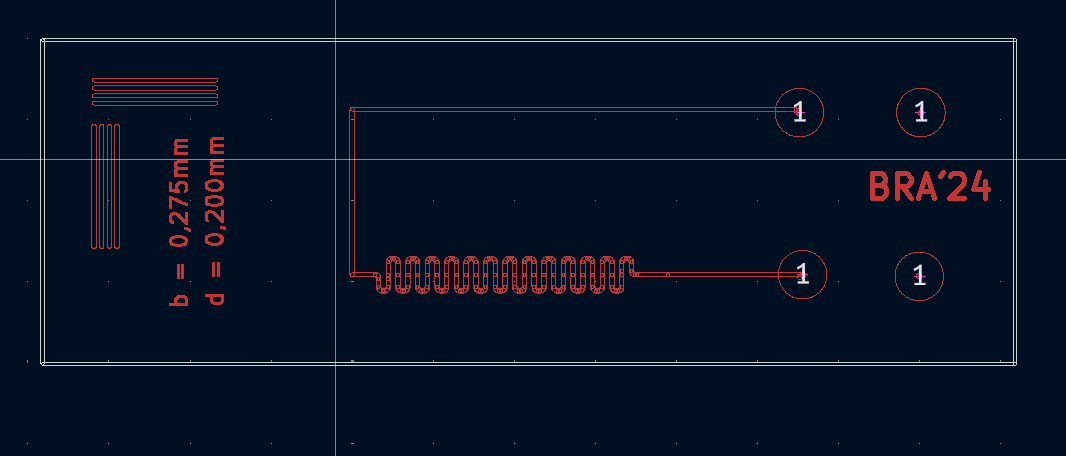
\includegraphics [width=\linewidth, height=6cm]{\figdir/PCB-Layout breite 0,275mm.png}
\caption{PCB Layout der Platine mit Leiterbahn = 0,275 mm}
\label{fig:Abbildung 1}
\end{figure}

\noindent
Außerdem wird der Name des Studierenden zusammen mit der Jahreszahl auch als Kupferbahn ausgeführt.
Bei der herkömmlichen Fertigung von Leiterplatten wird ein Bestückungsdruck für Bezeichnung der Komponenten und zusätzlichen Informationen zu den Bauteilen verwendet.
Da hier allerdings nur eine Kupferschicht vorgesehen ist, wird darauf verzichtet.
\\
Für die nachfolgende Messung bzw. Überprüfung unter dem Mikroskop werden vier Linien horizontal und vertikal in festem Abstand auf der Leiterplatte definiert.

\begin{figure}[h]
\centering 
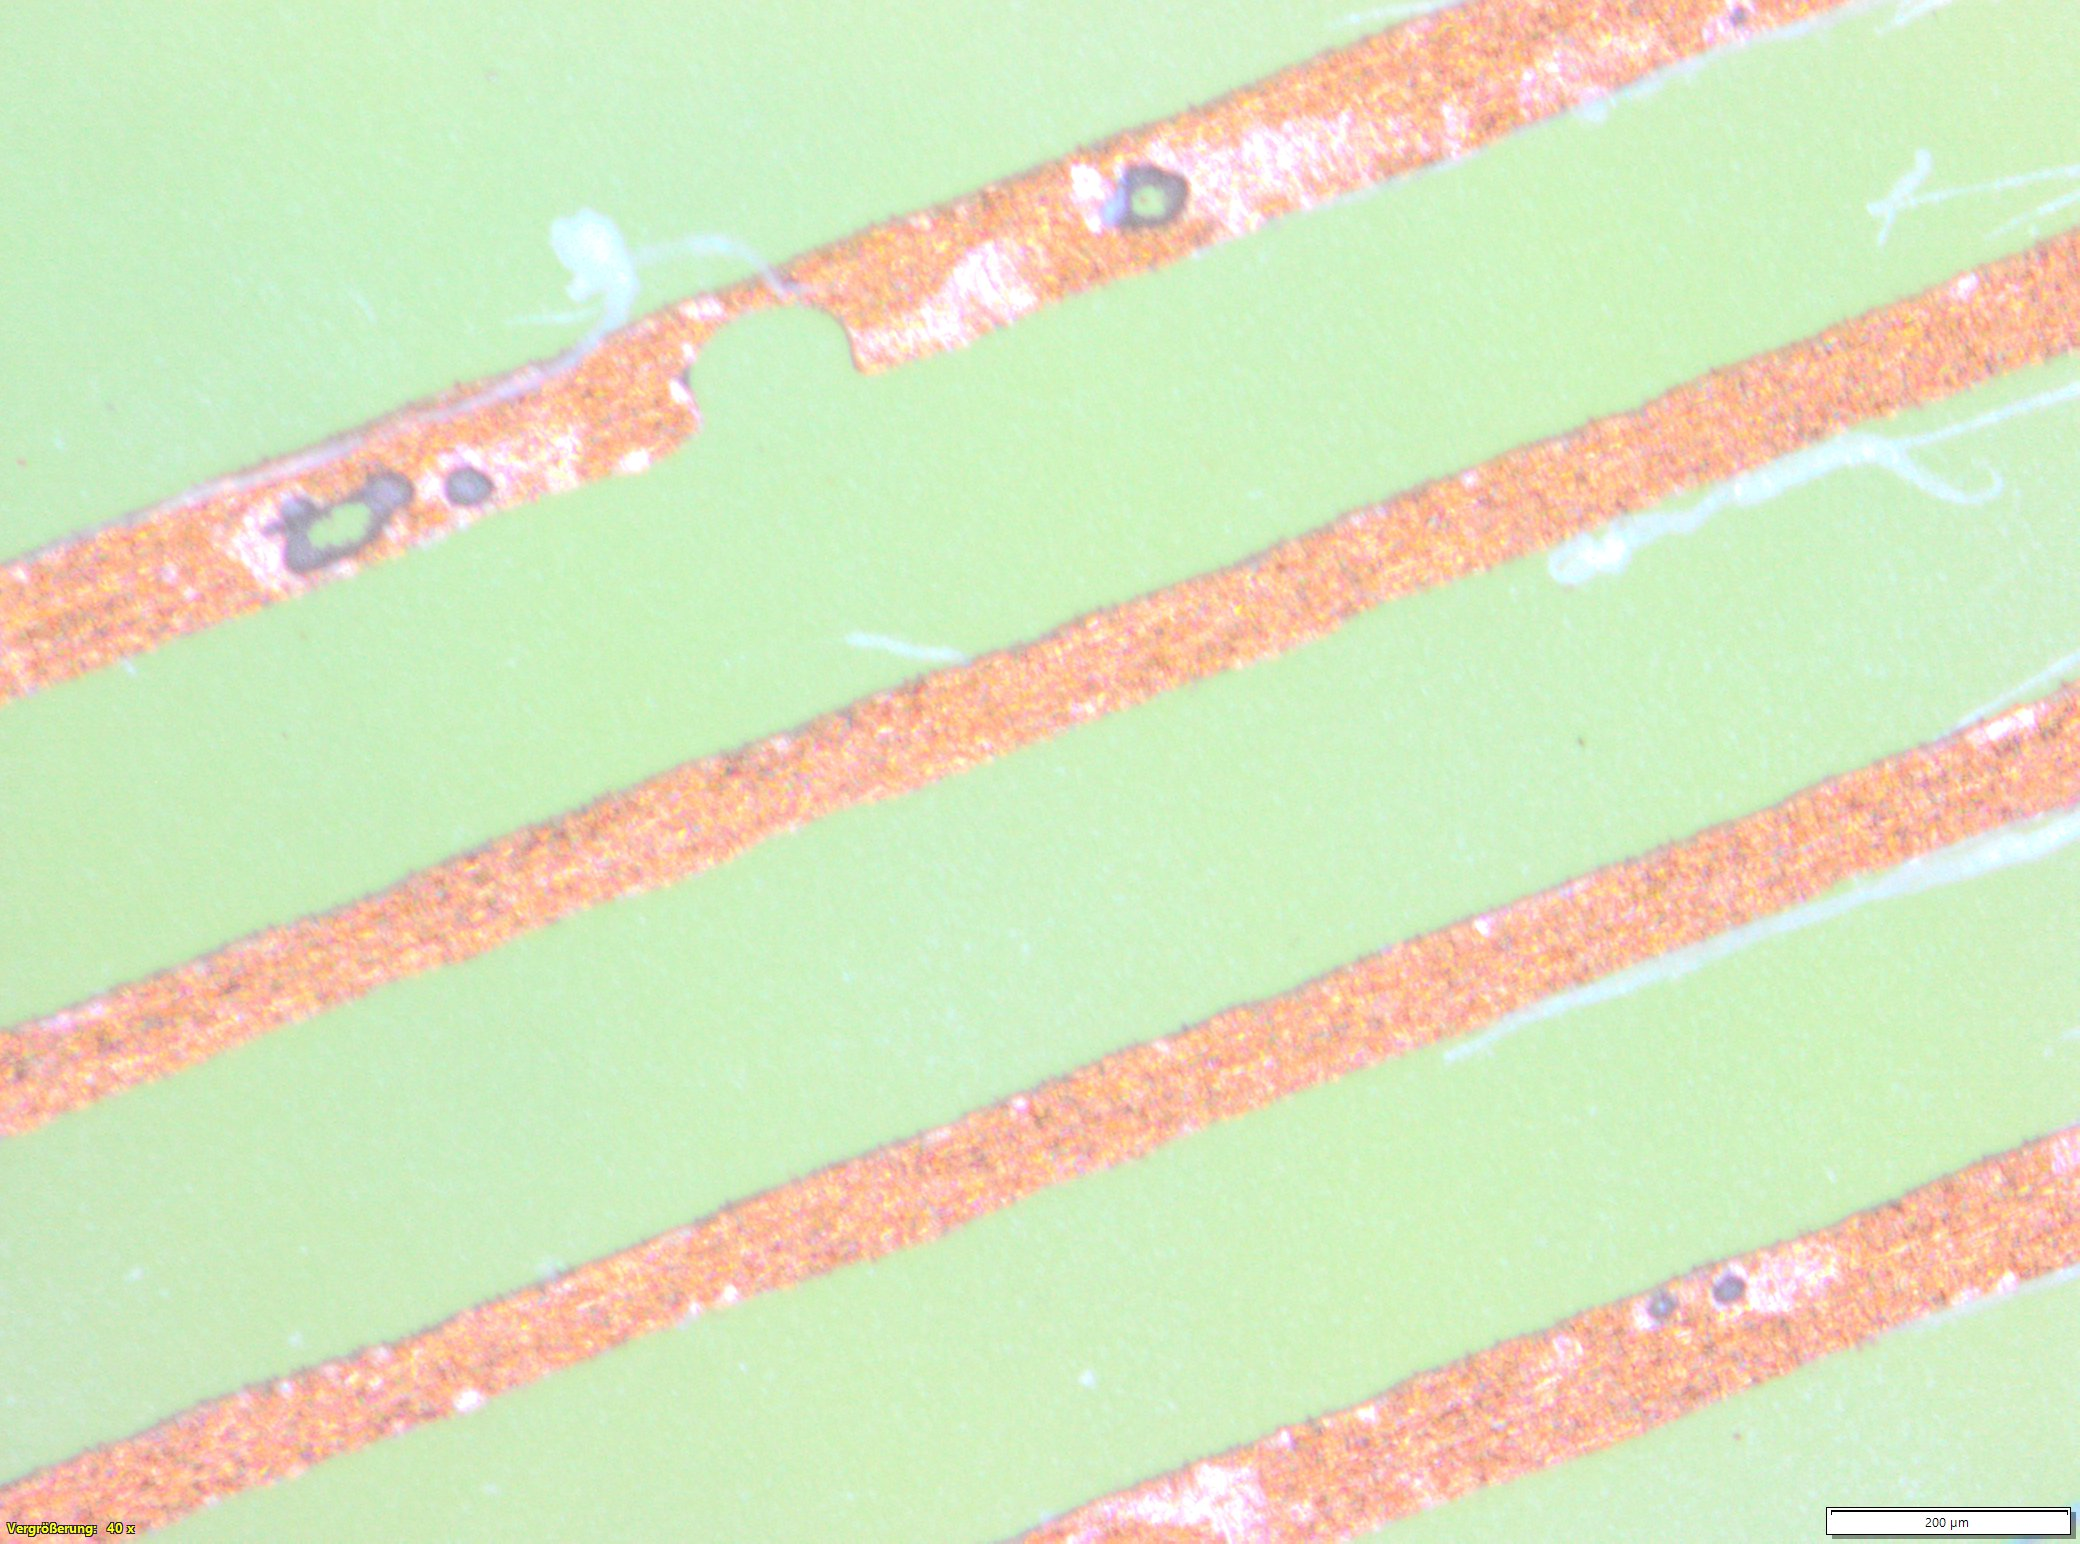
\includegraphics [width=12cm ,height=6cm]{\figdir/Mikroskopie_paralleleLeiterbahn}
\caption{parallele Leiterbahnen unter Mikroskop}
\label{fig:Abbildung 2}
\end{figure}

\noindent
Die Ursachen für Fehler auf den geätzten Leiterbahnen sind vielschichtig.
So können beispielsweise Ungenauigkeiten beim Belichten oder Staub auf der Maske zu unpräzisen Strukturen führen.
Während des Entwicklungsprozesses können ungleichmäßige Ergebnisse durch unvollständige oder fehlerhafte Prozesse entstehen.
Im Ätzprozess selbst können Probleme wie unzureichende Ätzlösung, Lufteinschlüsse, Überätzung oder ungleichmäßiger Materialabtrag auftreten.
Um derartige Fehler zu vermeiden, bedarf es einer sauberen Arbeitsumgebung sowie optimierter Prozessparameter.

\subsection{Herstellung der Platine}
Für die Herstellung von Leiterplatten existieren diverse Verfahren.
An der Hochscule wird das Ätzverfahren eingesetzt wird.
Dieses besteht aus den drei Hauptschritten Belichten, Entwickeln und Ätzen.
Darüber hinaus sind mehrere Vor- und Nachbearbeitungsschritte erforderlich, um eine optimale Verarbeitung zu gewährleisten.\\
\\
Um das Material effizient zu nutzen und Produktionsabfälle zu minimieren, werden mehrere Leiterplatten zu einer Einheit zusammengefasst, die als Nutzen bezeichnet wird.
Ein solcher Nutzen entspricht der Größe einer Europlatine, was eine standardisierte und platzsparende Anordnung ermöglicht.\\
\\
Die Belichtungsmaske für den Nutzen wird durch Bedrucken einer transparenten Folie mit einem Laserdrucker erstellt.
Um eine gleichmäßige Lichtundurchlässigkeit sicherzustellen, werden zwei identische Folien exakt übereinander geklebt.
Dies gewährleistet eine hohe Präzision beim Belichten und damit eine gute Qualität der späteren Leiterplatten.\\
\\
Nach dem Ätzen sind die Platinen noch als Teil des Europlatinen-Nutzens verbunden und müssen im Anschluss voneinander getrennt werden.
Der Trennvorgang erfolgt mithilfe einer Hebelschere.
Die Verwendung dieses Werkzeugs ermöglicht ein sauberes und präzises Zuschneiden der einzelnen Platinen.\\

\subsubsection{Belichten}
Beim Ätzverfahren wird die Platine mit einem Ätzresistlack versehen, der an bestimmten Stellen durch Belichtung seine Schutzfunktion verliert. Um dies zu ermöglichen, wird die auf dem Rohling befindliche Schutzfolie der Ätzresistschicht entfernt. Danach wird die Belichtungsmaske exakt auf dem Rohling positioniert.\\
\\
Damit die Belichtungsmaske während des Belichtungsvorgangs nicht verrutscht, verfügt das Belichtungsgerät über eine Vakuumfolie, die die Maske sicher auf dem Rohling fixiert. Für eine Standardleiterplatte beträgt die Belichtungsdauer etwa 2 Minuten. Während dieser Zeit bleibt der UV-Belichtungsapparat geschlossen, um eine gleichmäßige Belichtung zu gewährleisten.\\
\\
Nach der Belichtung sollte der Rohling mit der Maske etwas abkühlen, bevor die Belichtungsmaske entfernt wird. Es ist jedoch wichtig, den nächsten Schritt so schnell wie möglich durchzuführen, da das Ätzresist bei Tageslicht weiter belichtet werden kann. Dies könnte dazu führen, dass ungewollte Bereiche ihre Schutzwirkung verlieren und Fehler im weiteren Herstellungsprozess auftreten.

\begin{figure}[h]
\centering 
\includegraphics [width=12cm ,height=5.5cm]{\figdir/Belichtungsmaske und Gerät}
\caption{Belichtungsmaske und Gerät}
\label{fig:Abbildung 3}
\end{figure}

\subsubsection{Entwickeln}
Im Rahmen des Entwicklungsprozesses der Platine wird diese zunächst in einen Rahmen eingespannt und in eine Kammer gebracht, in der sie mit einer Lösung von Natriumhydroxid besprüht wird.
Das Besprühen ist auf etwa eine Minute zu beschränken, wobei bereits nach 15 bis 20 Sekunden erste Ergebnisse sichtbar sein sollten.\\
\\
Nach Ablauf der Minute wird der Entwicklungsprozess durch Erhitzen in einem Wasserbad gestoppt.
Im Anschluss werden die verbliebenen Rückstände unter fließendem Wasser abgespült, um eine vollständige Reinigung der Oberfläche zu gewährleisten.\\
\\
Nach diesem Schritt sollten die ungeschützten Kupferflächen sichtbar werden, die im darauffolgenden Prozess durch Ätzen entfernt werden.\\
Für ein fehlerfreies Ergebnis ist es entscheidend, dass die Natronlauge frisch, leicht erhitzt und im korrekten Mischverhältnis verwendet wird.\\

\begin{figure}[h]
\centering 
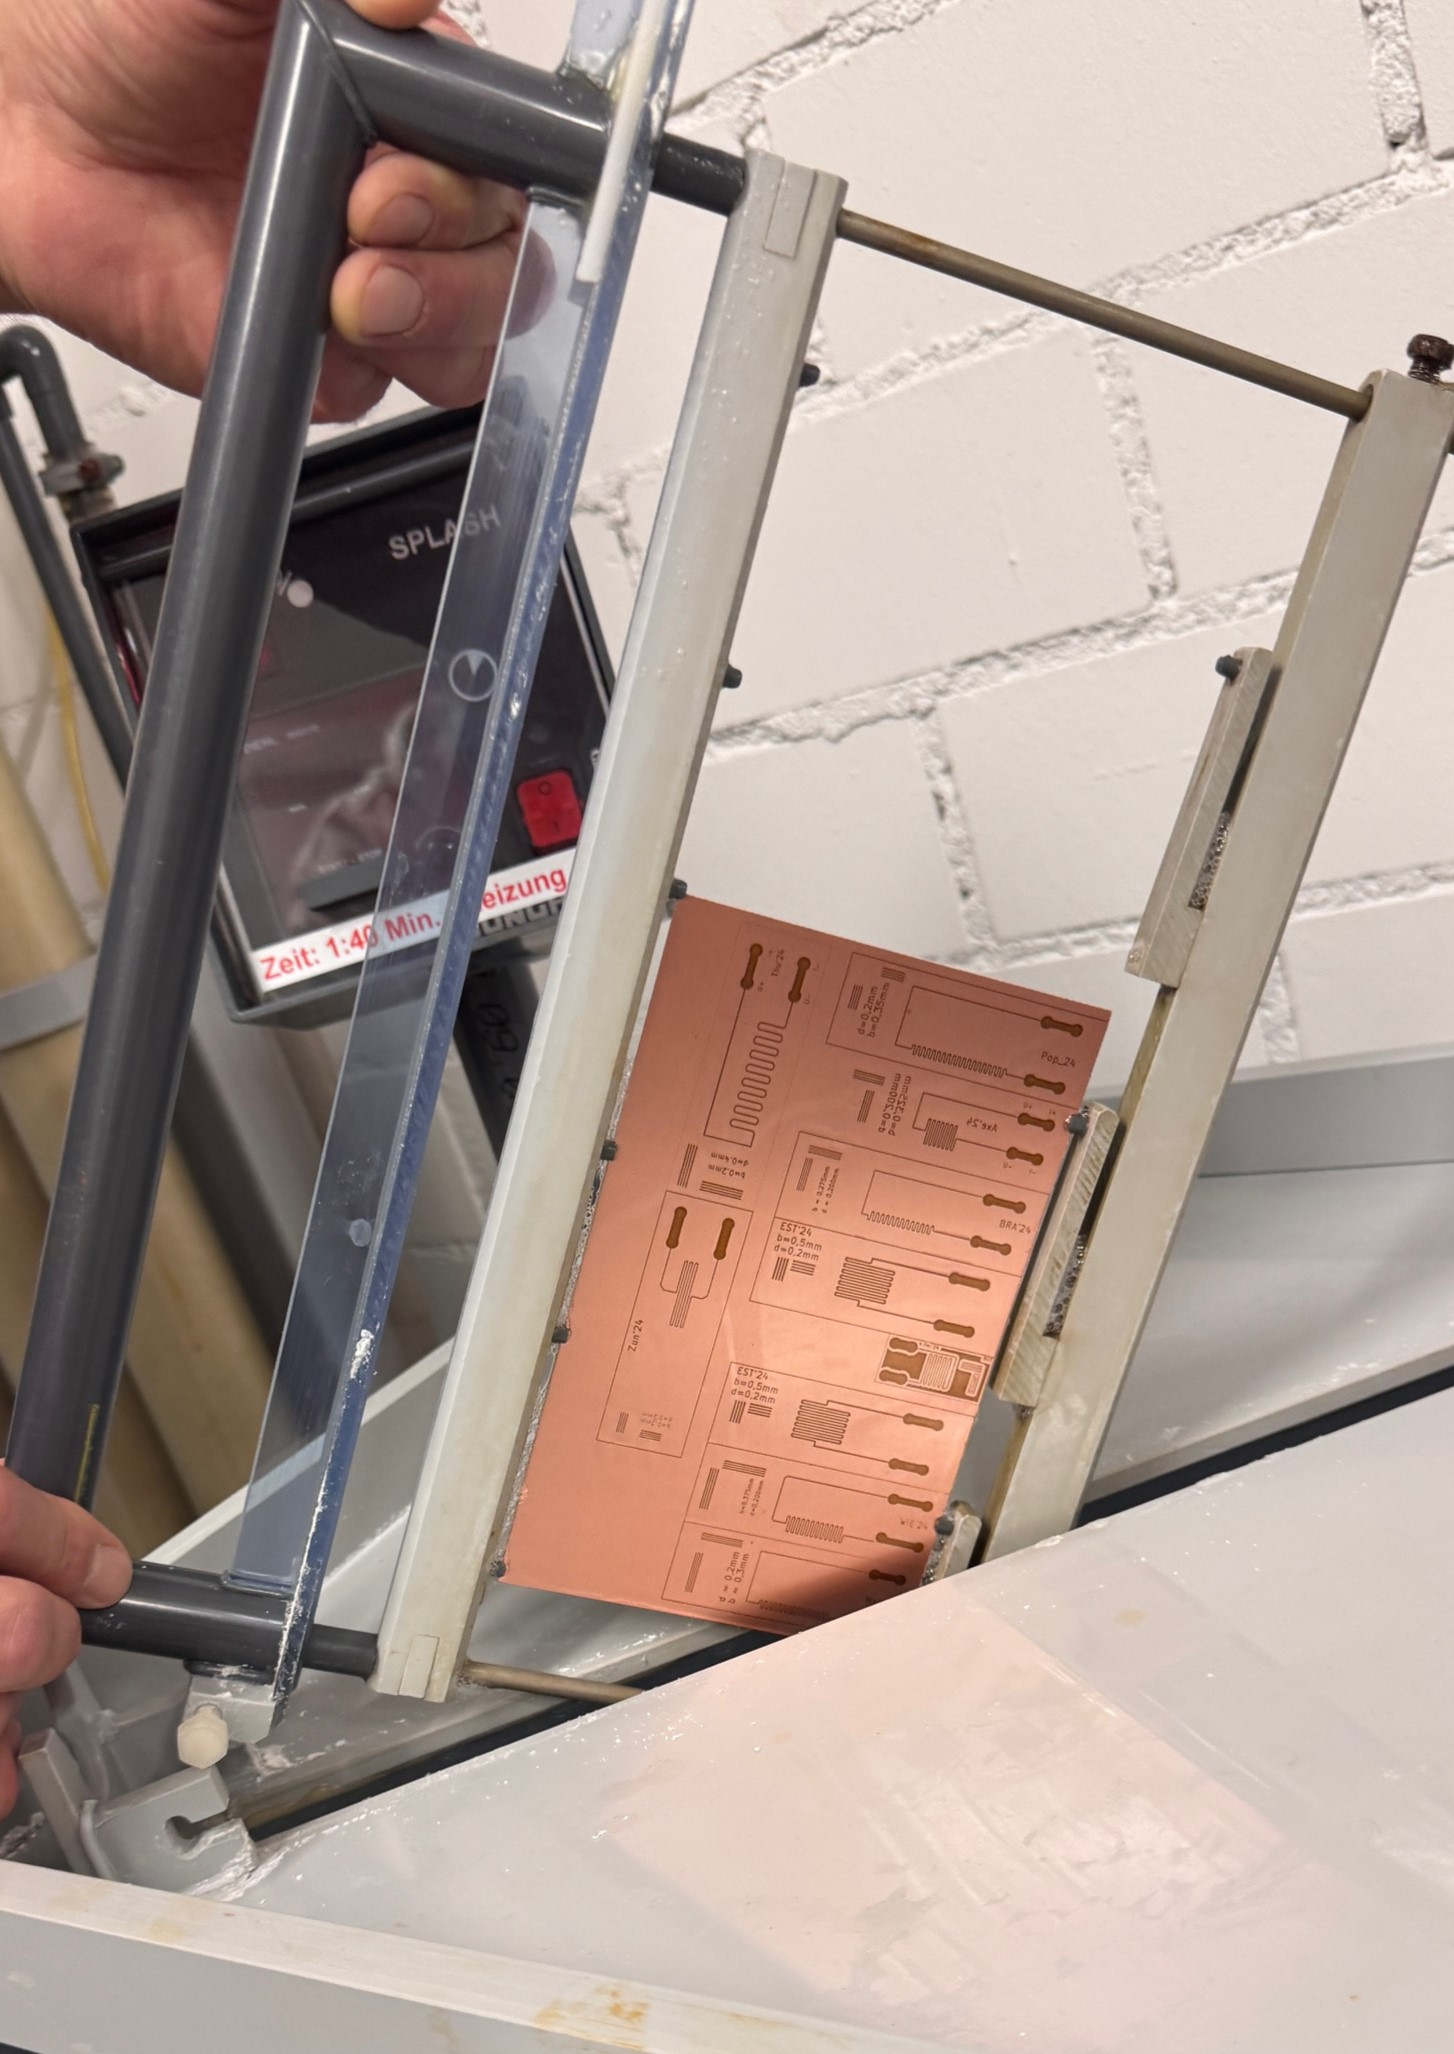
\includegraphics [width=12cm ,height=8cm]{\figdir/Leiterbahn nach Entwickeln}
\caption{Leiterbahn nach Entwickeln}
\label{fig:Abbildung 4}
\end{figure}

\subsubsection{Ätzen}
Für den Ätzvorgang wird die Platine erneut in einen Rahmen eingespannt und in einer Kammer mit Eisen-III-Chlorid-Lösung besprüht.
Die Ätzdauer beträgt ca. 3 Minuten, wobei die ungeschützten Kupferbereiche gezielt vom Ätzmittel entfernt werden.
Im Anschluss wird die Platine in einem Wasserbad vorgereinigt, um verbleibende Rückstände des verwendeten Ätzmittels zu entfernen.
Abschließend wird die Platine unter fließendem Wasser gründlich abgespült.
Abschließend wird die Leiterplatte getrocknet und für die weitere Verarbeitung vorbereitet.\\
\\
Während des Ätzvorgangs können jedoch Fehler aus dem Entwicklungsprozess sichtbar werden.
Ein unzureichend entwickeltes Ätzresist zeigt sich daran, dass die Kupferschichten nach den ersten 30 Sekunden nicht die typische hellrosa Verfärbung aufweisen.
Dies kann auf eine unzureichende Auftragung oder eine fehlerhafte Entwicklung des Resists zurückzuführen sein, was wiederum ungewollten Materialabtrag und fehlerhafte Leiterbahnen zur Folge haben kann.

\subsubsection{Nachbearbeitung}
Nach dem Ätzen erfolgt das Bohren der Löcher in die Platine.
Dabei entsteht Epoxidharzstaub, der als gesundheitsschädlich und potenziell krebserregend einzustufen ist.
Um die Belastung durch diesen Staub zu vermeiden, ist der Einsatz einer effektiven Absaugung zwingend erforderlich.
In diesem Praktikum wurde dieser Bearbeitungsschritt ausgelassen, da keine funktionalen Leiterplatten hergestellt wurden.\\
\\
Nach Abschluss dieses Prozesses kann die Leiterplatte mit Bauteilen bestückt und verlötet werden.
Für die erste Platine werden hierbei lediglich Testpunkte aufgelötet, um die Funktionsfähigkeit zu überprüfen.
Abschließend wird die Leiterplatte durch das Auftragen eines Schutzlacks vor Korrosion geschützt.
Auch diese Schritte wurden im Rahmen des Praktikums nicht durchgeführt.

\newpage
\section{KiCad Workshop}  

\subsection{Bibliotheken}  
Für die Entwicklung von Leiterplatten sind Bauteile und die dazugehörigen Footprints essenziell.
Diese werden in Libraries, auch Bibliotheken genannt, organisiert. Entwickler können projektbezogene Bibliotheken erstellen oder auf allgemeine Libraries zugreifen.
In der Industrie wird oftmals vorgegeben, wie Bauteile in das System eingepflegt werden müssen.\\  
\\
Das Erstellen eigener Bibliotheken hat den Vorteil, dass der Entwickler sich schneller zurechtfindet.
Zudem verwenden Leiterplattenhersteller oft ein festgelegtes Sortiment an Bauteilen.
In solchen Fällen ist es sinnvoll, Bibliotheken speziell für bestimmte Zulieferer anzulegen.  

\begin{figure}[h]  
    \centering  
    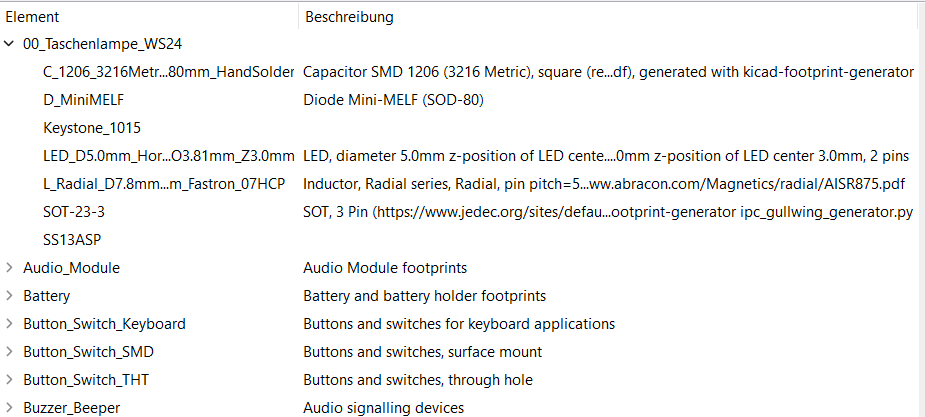
\includegraphics[width=0.8\textwidth]{\figdir/Footprint_Bibliothek mit Bauteilen.png}  
    \caption{Darstellung einer Bibliothek mit Bauteilen.} 
    \label{fig:Abbildung 5} 
\end{figure}  

\subsubsection{Bauteile}  
Ein Schaltplan bildet die Grundlage für jede Leiterplatte.
Die dafür benötigten Bauteile können aus den KiCad-Standardbibliotheken übernommen oder individuell erstellt werden.
Im Workshop wurden alle Bauteile in einer eigenen Bibliothek angelegt, um den Projekt Anforderungen zu entsprechen.\\
\\
Bauteile werden im Bauteileditor erstellt, wobei Eigenschaften wie Artikelnummern, Datenblätter oder 3D-Modelle hinterlegt werden können.
Um Zeit zu sparen, können bestehende Bauteile kopiert und angepasst werden.  

\begin{figure}[h]  
    \centering  
    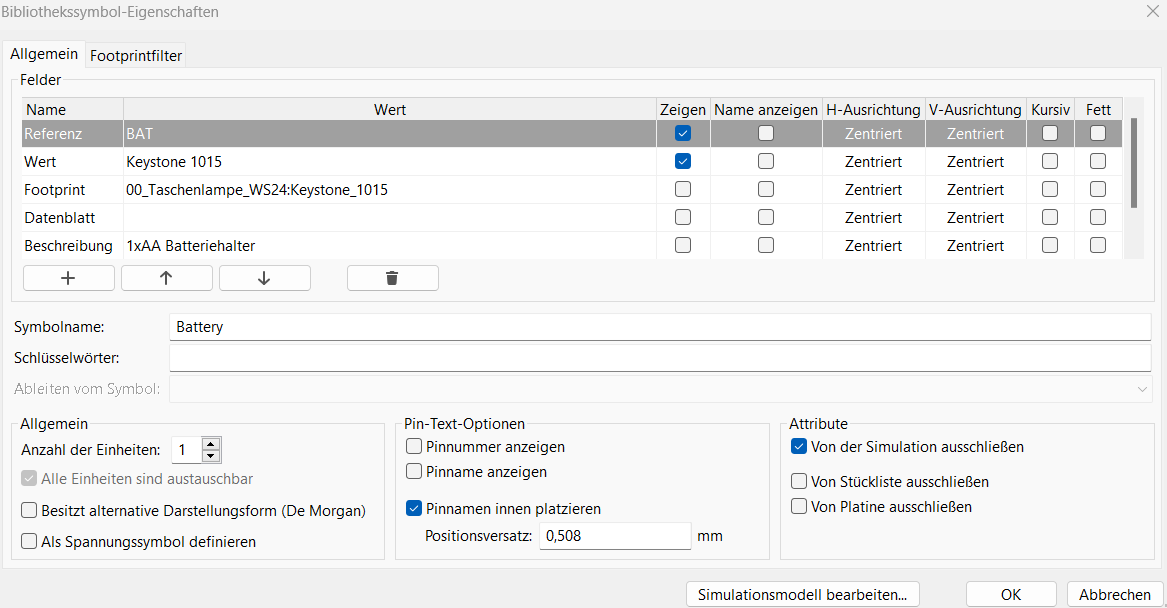
\includegraphics[width=0.8\textwidth, height=5cm]{\figdir/Battery_Symbol Eigenschaften.png}  
    \caption{Eigenschaften eines Bauteils}  
    \label{fig:Abbildung 6}
\end{figure}  

\noindent
Bauteile lassen sich im Bauteileditor entweder komplett neu erstellen oder durch Kopieren bestehender Bauteile zeitsparend anpassen, um sie den individuellen Anforderungen anzupassen.\\
Der folgende Batterie-Halter wurde beispielsweise aus einem Datenblatt übernommen und anschließend entsprechend modifiziert.

\begin{figure}[h]  
    \centering  
    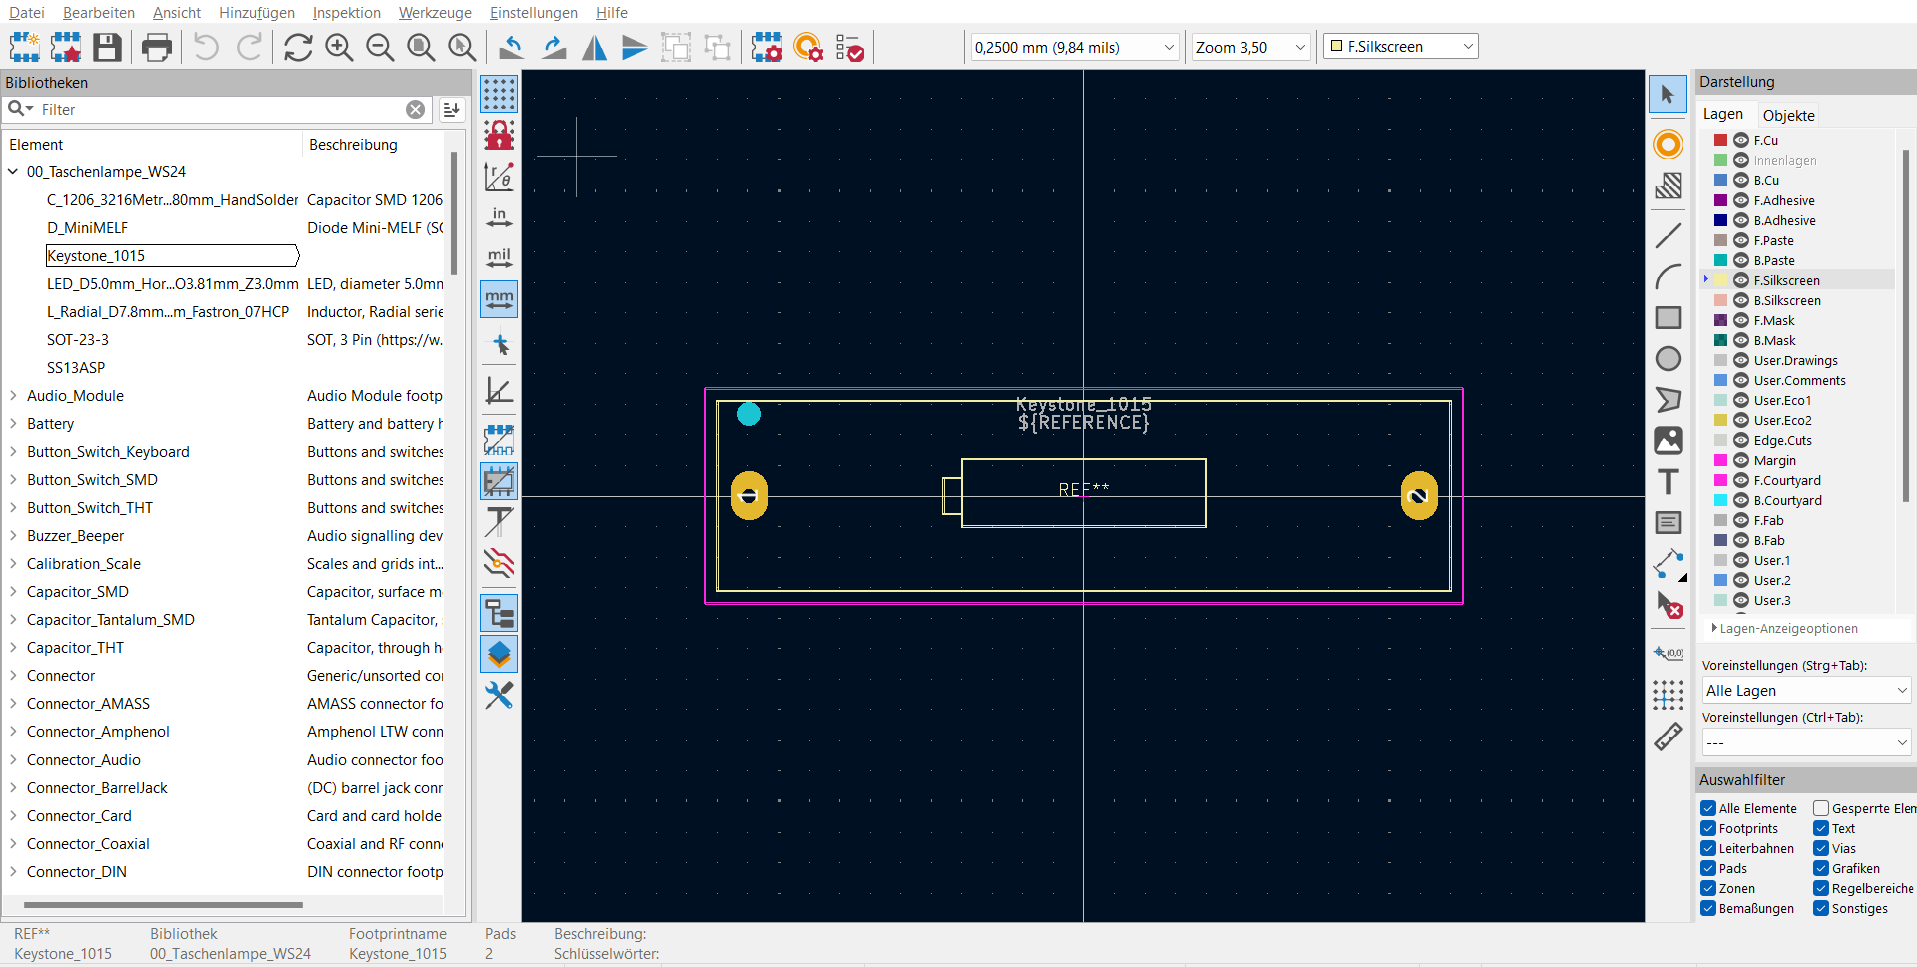
\includegraphics[width=0.8\textwidth, height=5cm]{\figdir/Footprinteditor.png}  
    \caption{Erstellung eines Bauteils im Bauteileditor} 
    \label{fig:Abbildung 7} 
\end{figure}  

\newpage

\subsubsection{Footprints}  
Footprints stellen die Verbindung zwischen den Bauteilen und der Leiterplatte her. Sie werden im Footprinteditor erstellt und repräsentieren den "Fußabdruck"{}eines Bauteils auf der Platine.\\
\\
Die Verbindung erfolgt über Lötpads, die an die Bauteilkontakte angepasst sind. Für das Handlöten sollten Lötpads größer gestaltet werden, um die Bearbeitung zu erleichtern.
Bei automatischer Bestückung sollten die Pads so klein wie möglich gehalten werden, um Platz zu sparen und den sogenannten Gravestone-Effekt (Aufstellen der Bauteile) zu verhindern.  

\begin{figure}[h]  
    \centering  
    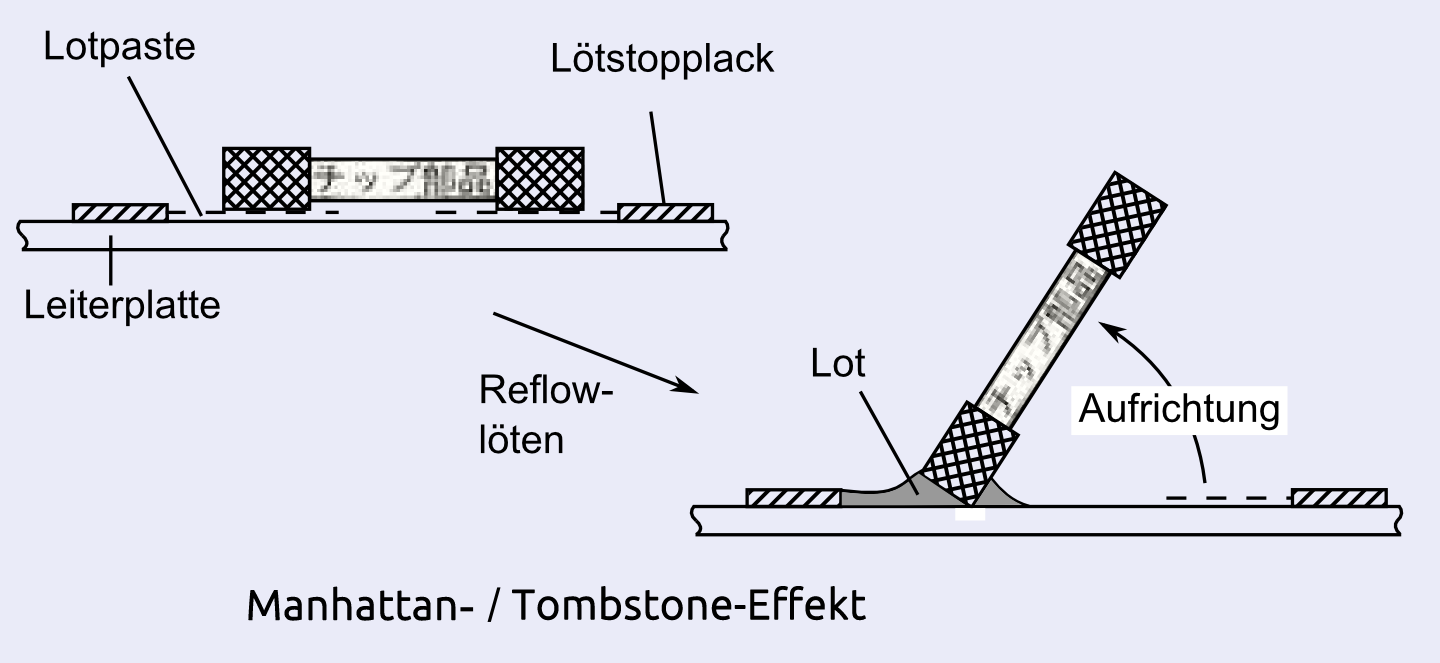
\includegraphics[width=0.6\textwidth, height=4.5cm]{\figdir/Gravestone_Effekt.png}  
    \caption{Gravestone-Effekt: Aufstellen der Bauteile\cite{almit_grabstein_manhattan}}
    \label{fig:Abbildung 8}  
\end{figure}  
\newpage

\subsection{Erstellen des Schaltplans}  
Nach dem Einpflegen der Bauteile wird der Schaltplan im Schaltplan-Editor erstellt. Die Bauteile werden aus der Bibliothek eingefügt, positioniert und miteinander verbunden. Netzklassen können definiert werden, um Abstände zwischen Signalen oder Gruppen (z. B. Last- und Steuerkreis) zu berücksichtigen.\\  
\\
Um die Übersichtlichkeit zu erhöhen, können Textvariablen und Labels genutzt werden. Im Workshop wurden Labels beispielsweise für Ground (GND) eingesetzt.  

\begin{figure}[h]  
    \centering  
    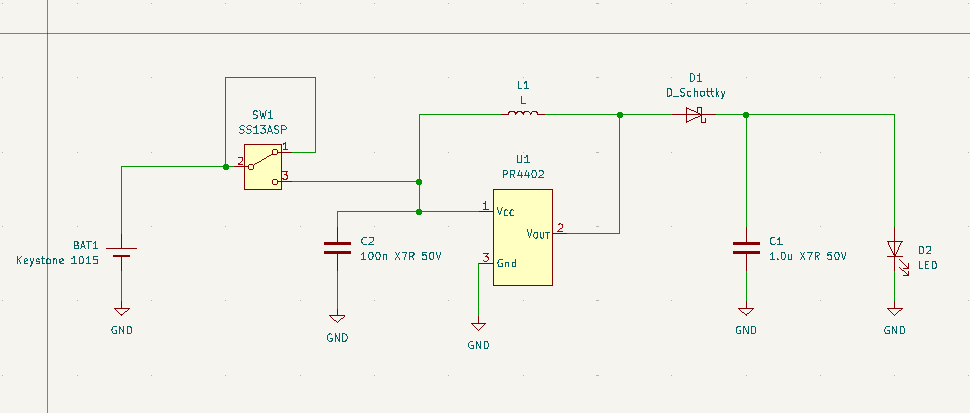
\includegraphics[width=0.8\textwidth]{\figdir/Schaltplan_Taschenlampe.png}  
    \caption{Schaltplan der Taschenlampe mit markierten Labels.}  
    \label{fig:Abbildung 9}
\end{figure}  

\noindent
Wird während der Schaltplanerstellung festgestellt, dass ein Footprint nicht zugewiesen wurde, so kann dies direkt im Schaltplaneditor nachgeholt werden.\\ 
Zur Bearbeitung von Footprints oder Bauteilen kann ebenfalls direkt aus dem Schaltplaneditor in den Footprint- bzw. Bauteileditor gewechselt werden.\\
\\
Während und nach der Schaltplanerstellung sollte ein ERC („Electrical Rule Check“) durchgeführt werden. Dieser Prüfvorgang analysiert den Schaltplan auf Fehler und gibt entsprechende Meldungen aus.
Neben Fehlern können auch Warnungen auftreten, die sich häufig auf Labels oder Netzklassen beziehen. Warnungen sind oft weniger kritisch.
Fehler sollten jedoch nie ohne sorgfältige Prüfung ignoriert werden.
Sollte ein gemeldeter Fehler tatsächlich keinen Einfluss auf die Funktion haben, so kann er im ERC entsprechend markiert und zukünftig ausgeblendet werden.

\newpage

\subsection{Erstellen des Platinenlayouts}  
Das Layout ist die Umwandlung des Schaltplans in eine physische Leiterplattenstruktur. Dabei werden die Footprints der Bauteile auf der Platine positioniert und durch Leiterbahnen verbunden.\\

Der Layoutprozess umfasst die folgenden Schritte:  
\begin{itemize}  
    \item Festlegung der Platinenabmessungen.  
    \item Positionierung der Footprints im Bauraum.  
    \item Manuelles Routen der Leiterbahnen.  
\end{itemize}  

\noindent
Ein durchgehendes GND-Potenzial wird als Kupferschicht ausgeführt. Die restlichen Verbindungen werden manuell erstellt. Dabei ist besonders darauf zu achten, dass die GND-Schicht nicht unterbrochen wird und die Footprints keine Überschneidungen aufweisen.  

\begin{figure}[h]  
    \centering  
    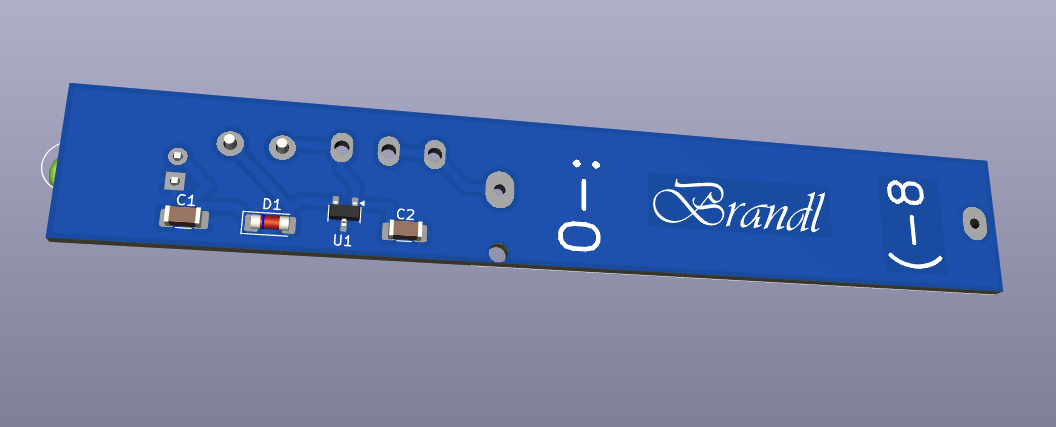
\includegraphics[width=0.8\textwidth]{\figdir/3D_Betrachter_Taschenlampe}  
    \caption{3D Layout Rückseite mit Bauteilen.} 
    \label{fig:Abbildung 10} 
\end{figure}  

\noindent
Die Leiterplatte erhält abschließend einen Bestückungsdruck (Silkscreen), der die Bauteilpositionen markiert.
Dieser kann auch mit optischen Markierungen noch erweitert werden, um das Platinendesign künstlerisch zu gestalten



\newpage
\section{Endmontage Radio und Taschenlampe}

\subsection{Bestücken und Löten der Taschenlampe}
Die Taschenlampe wurde speziell so gestaltet, dass selbst die SMD-Bauteile problemlos von Hand gelötet werden können. Dabei spielt insbesondere die Größe der Lötpads eine entscheidende Rolle. Während für das Löten im Reflow-Ofen möglichst kleine Pads verwendet werden, müssen diese für das manuelle Löten etwas größer ausgelegt sein, um genügend Spielraum für den Lötkolben zu gewährleisten.

Zu Beginn wurden die SMD-Bauteile auf der Unterseite der Platine gelötet. Diese Reihenfolge erleichtert die Arbeit, da die Platine dadurch weiterhin flach auf der Arbeitsfläche aufliegt, was die präzise Positionierung der kleinen Bauteile unterstützt. Im Anschluss daran wurden die Durchsteckbauteile gelötet. Diese Arbeitsschritte sind in der Regel einfacher, da die größeren Bauteile stabiler sind und während des Lötprozesses nicht verrutschen können.

Nach dem Löten der bedrahteten Bauteile wurden überstehende Drähte, beispielsweise von Leuchtdioden und Spulen, mithilfe eines Seitenschneiders entfernt.

Bei der Montage der Taschenlampe ist es wichtig, die Reihenfolge einzuhalten: Zuerst werden SMD-Bauteile und anschließend Durchsteckbauteile gelötet. Besondere Aufmerksamkeit gilt der Polarität der Schottky-Diode und der Leuchtdioden. Zudem sollten Kondensatoren nicht übermäßig lange mit Hitze in Kontakt kommen, um Schäden zu vermeiden.

Nach Abschluss des Lötprozesses wird die Taschenlampe auf ihre Funktion überprüft.

\begin{figure}[h!]
    \centering
    \includegraphics[width=0.8\textwidth]{platzhalter_taschenlampe_unterseite.png}
    \caption{Unterseite der Taschenlampe mit sichtbaren SMD-Bauteilen.}
    \label{fig:taschenlampe_unterseite}
\end{figure}

\begin{figure}[h!]
    \centering
    \includegraphics[width=0.8\textwidth]{platzhalter_taschenlampe_oberseite.png}
    \caption{Oberseite der Taschenlampe mit Schalter, Batteriehalter, Spule und LED.}
    \label{fig:taschenlampe_oberseite}
\end{figure}

\subsection{Bestücken und Löten des Radios}
Die Radioplatine wurde mit einer Kombination aus manuellen und maschinellen Verfahren bestückt. Auch beim Auftragen der Lötpaste kamen unterschiedliche Methoden zum Einsatz.

Auf der Vorderseite der Radioplatine befinden sich sechs Leuchtdioden und zwei Lautsprecher. Wegen der vergleichsweise geringen Bauteilanzahl wurde die Lötpaste hier mit einem Handdispenser aufgetragen, der über Druckluft gesteuert wird. Ein Fußpedal reguliert den Luftdruck und sorgt dafür, dass eine präzise Menge Lötpaste auf die Pads aufgetragen wird. Bei den Lautsprecherpads wird die Paste in Mäanderbewegungen verteilt, während bei den Pads der Leuchtdioden einzelne Linien ausreichen.

\begin{figure}[h!]
    \centering
    \includegraphics[width=0.8\textwidth]{platzhalter_handdispenser.png}
    \caption{Handdispenser beim Auftragen der Lötpaste auf die Radioplatine.}
    \label{fig:handdispenser}
\end{figure}

Nach dem Auftragen der Lötpaste erfolgte die Bestückung der Bauteile mit einem Handmanipulator. Dieser erkennt durch Anpressdruck, wann ein Bauteil aufgenommen oder aufgesetzt wird, und nutzt Unterdruck, um die Bauteile sicher zu halten. Zusätzlich ermöglicht der Manipulator das Drehen der Bauteile, während ein rotierendes Magazin für eine kontinuierliche Versorgung sorgt.

\begin{figure}[h!]
    \centering
    \includegraphics[width=0.8\textwidth]{platzhalter_manipulator.png}
    \caption{Aufnahme eines Elko-Kondensators mit dem Manipulator.}
    \label{fig:manipulator}
\end{figure}

Anschließend wurde die Vorderseite der Radioplatine in einem Reflow-Ofen verlötet. Die Vorheizphase dauerte 45 Sekunden, gefolgt von einer 15-sekündigen Lötphase. Nach dem Löten musste die Platine zunächst auskühlen, da sie sehr heiß war. Um ein Verrutschen der bereits gelöteten Bauteile beim zweiten Lötvorgang zu verhindern, wurden diese zusätzlich mit Kleber fixiert.

Für die Rückseite der Platine wurde die Lötpaste mit einer Schablone und einer Rakel aufgetragen. Dabei musste die Platine exakt unter der Schablone positioniert werden, um sicherzustellen, dass die Paste präzise auf den Pads landet.

\begin{figure}[h!]
    \centering
    \includegraphics[width=0.8\textwidth]{platzhalter_schablone.png}
    \caption{Schablone und Rakel beim Auftragen der Lötpaste auf die Rückseite der Platine.}
    \label{fig:schablone}
\end{figure}

Nach dem Auftragen der Paste wurde die Platine in einen Bestückungsautomaten eingelegt. Dieser erkannte die Fiducial Points und richtete die Platine entsprechend aus. Die meisten Bauteile wurden automatisch bestückt, jedoch mussten einige wie Elkos, bestimmte SMD-Widerstände, Kondensatoren und ICs manuell mit dem Manipulator ergänzt werden.

Für zwei ICs kam ein spezielles Kamerasystem zum Einsatz. Dieses verwendete Spiegel, um die Kontakte unterhalb der Chips sichtbar zu machen, was eine präzise Platzierung ermöglichte.

Nach der vollständigen Bestückung wurde die Radioplatine ein zweites Mal im Reflow-Ofen verlötet. Anschließend lötete man per Hand drei Drähte zum Programmieren des Radiochips an. Die Software wurde aufgespielt, eine Antenne an Stecker X201 befestigt, und die Funktionalität des Radios geprüft.

\begin{figure}[h!]
    \centering
    \includegraphics[width=0.8\textwidth]{platzhalter_reflowofen.png}
    \caption{Radioplatine im Reflow-Ofen.}
    \label{fig:reflowofen}
\end{figure}

\begin{figure}[h!]
    \centering
    \includegraphics[width=0.8\textwidth]{platzhalter_antenne.png}
    \caption{Rückseite der Radioplatine mit angeklemmter Antenne.}
    \label{fig:antenne}
\end{figure}


\newpage

\section{Fazit}
Das Praktikum in der Aufbau- und Verbindungstechnik bot eine umfassende Einführung in die Herstellung und das Design von Leiterplatten. \ldots


\newpage
\listoffigures % Abbildungsverzeichnis
\newpage

\section*{Quellenverzeichnis}
 
\end{document}
